\begin{figure}[htbp]
	% Partly taken from http://www.texample.net/tikz/examples/convolution-of-two-functions/
	\centering
	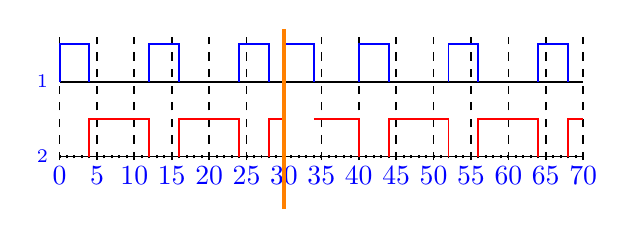
\begin{tikzpicture}[
		scale=0.095,
		line width=0.25mm,
		every node/.style={scale=1, text=blue},
		major tick/.style={semithick, dashed},
		x tick label/.style={anchor=north, minimum width=5mm},
		task1/.style={blue},
		task2/.style={red},
		task3/.style={green},
		desc/.style={anchor=east},
		konf/.style={orange, very thick}
		]
	
	% Task 2
	\draw (0, 0) -- (70, 0);
	\node[desc] at (0, 0) {$\uptau_2$};
	
	% Task 1
	\draw (0, 10) -- (70, 10);
	\node[desc] at (0, 10) {$\uptau_1$};	
	
	% Small ticks
	\foreach \x in {0, 1,...,70}{
		\draw (\x, -0.25) -- (\x, 0.25);
	}
	
	% Major ticks with label
	\foreach \x/\label in {0, 5,...,70}{
		\node[x tick label] at (\x, 0) {$\label$}; 		
		\draw[major tick] (\x, -0.5) -- (\x, 16);
	}
	
	% Draw all
%	\foreach \x in {0, 10,...,69}{
%		\draw[task1] (\x, 10) -- (\x, 15) -- (\x+4, 15) -- (\x+4, 10);
%	}

	\draw[task1] (0, 10) --  (0, 15) --  (4, 15) -- (4, 10);
	\draw[task2] (4, 0) --  (4, 5) --  (12, 5) -- (12, 0);
	\draw[task1] (12, 10) --  (12, 15) --  (16, 15) -- (16, 10);
	\draw[task2] (16, 0) --  (16, 5) --  (24, 5) -- (24, 0);
	\draw[task1] (24, 10) --  (24, 15) --  (28, 15) -- (28, 10);
	\draw[task2] (28, 0) --  (28, 5) --  (30, 5); % 2 done
	\draw[task1] (30, 10) --  (30, 15) --  (34, 15) -- (34, 10);
	\draw[task2] (34, 5) --  (40, 5) -- (40, 0);	
	\draw[task1] (40, 10) --  (40, 15) --  (44, 15) -- (44, 10);
	\draw[task2] (44, 0) --  (44, 5) --  (52, 5) -- (52, 0);
	\draw[task1] (52, 10) --  (52, 15) --  (56, 15) -- (56, 10);
	\draw[task2] (56, 0) --  (56, 5) --  (64, 5) -- (64, 0);
	\draw[task1] (64, 10) --  (64, 15) --  (68, 15) -- (68, 10);
	\draw[task2] (68, 0) --  (68, 5) --  (70, 5);
	
	\draw[konf] (30, 17) -- (30, -7);	
	
	\end{tikzpicture}
%	\caption{Ablaufübersicht}
\end{figure} 